% This is "sig-alternate.tex" V2.1 April 2013
% This file should be compiled with V2.5 of "sig-alternate.cls" May 2012
%
% This example file demonstrates the use of the 'sig-alternate.cls'
% V2.5 LaTeX2e document class file. It is for those submitting
% articles to ACM Conference Proceedings WHO DO NOT WISH TO
% STRICTLY ADHERE TO THE SIGS (PUBS-BOARD-ENDORSED) STYLE.
% The 'sig-alternate.cls' file will produce a similar-looking,
% albeit, 'tighter' paper resulting in, invariably, fewer pages.
%

\documentclass{sig-alternate}

\usepackage{listings}
\usepackage{graphicx}
\usepackage{amsmath}
\usepackage{algorithm2e}
\usepackage{csquotes}


\begin{document}


\title{Traffic-aware dynamic re-partitioning\\for a distributed key-value store}
\subtitle{CS848 - Fall 2016 Course Project}


\numberofauthors{1} 
\author{
	\alignauthor Vineet John\\
	\affaddr{David R. Cheriton School of Computer Science}\\
	\affaddr{University of Waterloo}\\
	\affaddr{Waterloo, Ontario, Canada}\\
	\email{vineet.john@uwaterloo.ca}
}


\maketitle
\begin{abstract}
Most modern data stores tend to be distributed, to enable the scaling of the data across multiple instances of commodity hardware. Although this ensures a near unlimited potential for storage, the data access is not always ideally partitioned, and the cost of a network round-trip may cause a degradation of end-user experience with respect to response latency. The problem attempted to be solved is to bring the data objects closer to the frequent sources of request using a dynamic re-partitioning algorithm. This is important if the objective is to mitigate the overhead of network latency, and especially so if the partitions are widely geo-distributed. The intention is to bring these features to an existing distributed key-value store product, Redis\cite{redis-website}.
\end{abstract}


\keywords{dynamic re-partitioning, key-value store, data placement}


\section{Introduction}

The objective for this project is to design a shared-something distributed architecture atop an existing key-value store that dynamically repartitions tuples based on usage metrics\\

This project is takes its roots in intelligent data placement, and in essence, attempts to delegate the data ownership to the distributed key-value store instance that is closest to the most frequent sources of a request, by implementing a web-service as an intermediary layer to the key-value store on each node. \\

The motivation of the project is three-fold:
\begin{itemize}
	\item Reduce the network latency by dynamic re-partitioning of the cached data based on usage heuristics. I.e. maximize the number of cache-hits on the local cache.
	\item Leveraging the same usage heuristics to selectively purge stale data.
	\item Optimizations need to be non-blocking so as to not interfere with the regular execution of fetch requests.
\end{itemize}


\section{Similar Work}
Attempts to identify ideal methods to dynamically partition data do exist. Two of them, SWORD\cite{quamar2013sword} and AdaptCache\cite{asad2016adaptcache}, rely on hyper-graphs to model the workload, and base the re-partitioning decisions off this model. SCHISM\cite{curino2010schism} relies on graph partitioning to find a predicate-based explanation of the partitioning strategy. E-store\cite{taft2014store} relies of a strategy of skewed placement, where the data placement decision is taken based on usage heuristics.\\

The system proposed in this document attempts to avoid expensive graph traversals and be able to log usage heuristics and perform a usage analysis in either constant or linear time. In addition, since Redis is widely used in industrial settings, it makes it an easier deployment strategy, compared to switching over to a new system. Also included is a web API for ease of data access, and minimize the overhead of having to implement a language specific client to interact with the caching layer.


\section{Model Assumptions}
The following assumptions are made, with respect to the system architecture and the problem being solved:
\begin{itemize}
	\item The load balancing layer on the application servers hosting the web-services ensures that the request from clients is served by the application server closest to the client. 
	\item The nature of the workload, as is the case with most caches, is pre-dominantly read requests.
	\item The network of nodes is geo-distributed
	\item Minimal memory usage on each of the nodes is a desirable property
	\item $ \displaystyle size(value) \gg size(key)$
\end{itemize}


\section{System Architecture}
This section elaborates on the components the system is comprised of, and explains the points of interaction between them. Figure \ref{fig:sysarch} shows a graphical representation of the architecture.\\

\begin{figure*}
\centering
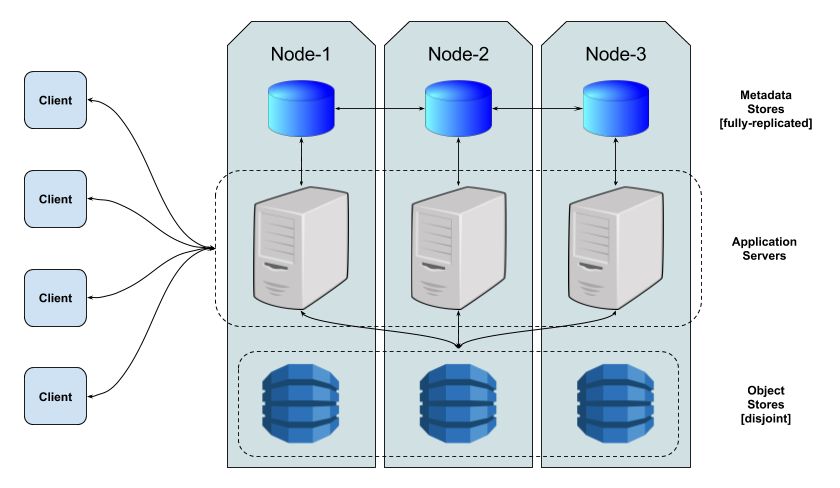
\includegraphics[width=\textwidth]{images/SystemArchitecture.png}
\caption{System Architecture}
\label{fig:sysarch}
\end{figure*}

\subsection{Components}
The components of the architecture are listed below:
\begin{itemize}
	\item \textbf{Web service layer:} This layer of abstraction over the ke-value store, is deployed on the application server nodes. It receives requests, reads placement details from the metadata layer and acts accordingly.
	\item \textbf{Metadata Layer:} This is a smaller key-value data store for metadata, which is a separate cluster running on the same nodes as the actual key-value stores. It stores the key metadata, like current placement, usage heuristics and recency of access.
	\item \textbf{Cache Layer:} This is the underlying in-memory datastore which the objects are primarily stored in. There is a single redis instance running on each of the nodes.
	\item \textbf{Placement Daemon:} This continuous process keeps running offline in periodic intervals to repartition the keys, based on the placement strategy described in algorithm \ref{algo-place}.
\end{itemize}

\subsection{Component Interaction}
Component Interaction can be enumerated as below:
\begin{itemize}
	\item The web service deployment instances are agnostic of each other.
	\item The metadata layer and the caching layer are agnostic of each other.
	\item A given web-service on node can initiate a key-value store request call on any of the instances in the cluster of nodes.
\end{itemize}


\section{Key concepts}
This section contains a description of the key concepts that the dynamic re-partioning strategy, is heavily dependant on, including the `Ownership coefficient' and the data format in which metadata for each key is maintained.

\subsection{Ownership coefficient}
The ownership coefficient (H) determines which nodes need to have a local copy of the data.\\

During the analysis phase of the data placement daemon, the key usage for each node is calculated using equation \ref{eq:1}:
\begin{equation*}g(O, x) = count(accesses\ on\ O)\ by\ host\ x \end{equation*}
\begin{equation} \label{eq:1} f(O,x) = \frac{g(O, x)}{g(O, \forall x)} \end{equation}

If equation \ref{eq:2} holds true, then node `x' is deemed eligible to possess a replicated copy of object O.
\begin{equation} \label{eq:2} f(O, x) - H \geq 0 \end{equation}

The above conditions operate under the constraint defined in equation \ref{eq:3}
\begin{equation} \label{eq:3} H - \frac{1}{n} \leq 0 \end{equation}
where `n' is the number of nodes in the architecture. This constraint is defined to avoid host starvation of key ownership, especially for cases in which hosts might 


\subsection{Metadata format}
The data object used to store the metadata for each tuple is given below. \textit{hosts} is a hashed set, \textit{hostAccesses} is a data-dictionary, and the numeric values are positive integers. \textit{lastAccessedDate} denotes when the key in question was last accessed, in terms of milliseconds elapsed since the epoch.
\begin{lstlisting}
{
    `totalAccessCount': 17,
    `hosts': [
        `ugster01.student.cs.uwaterloo.ca',
        `ugster03.student.cs.uwaterloo.ca'
    ],
    `hostAccesses': {
        `ugster01.student.cs.uwaterloo.ca': 9,
        `ugster02.student.cs.uwaterloo.ca': 3,
        `ugster03.student.cs.uwaterloo.ca': 5
    },
    `lastAccessedDate': 1480725771235
}
\end{lstlisting}


\section{Algorithmic Approach}
This section describes the algorithms being used to implement the architecture, including fetching, storing and re-partitioning tuples.\\

\subsection{Fetching tuples}
The algorithm to fetch tuples is described in algorithm \ref{algo-fetch}.

\begin{algorithm}
\KwData{key}
\KwResult{value/null}
\DontPrintSemicolon 
\;
query metadata data for key\;

\uIf{$metadata == null$}{
	return null;
}
\uElse{
	$owner\_hosts = metadata.hosts$\;
	\uIf{$current\_host \in owner\_hosts$}{
		make local request to get data\;
	}
	\uElse{
		make remote request\\
		(incurring additional latency)\;
	}
	spawn thread and collect access metrics\;
}
\;
\label{algo-fetch}
\caption{Fetching values}
\end{algorithm}


\subsection{Storing tuples}
The algorithm to store tuples is described in algorithm \ref{algo-store}.

\begin{algorithm}
\KwData{key, value}
\KwResult{success = true/false}
\DontPrintSemicolon 
\;
query metadata data for key;\\

\uIf{metadata == null}{
	store new key and value locally;
	generate metadata object;
	post metadata object to metadata layer;
}
\uElse{
	$owner-hosts = metadata.hosts$\;
	\uIf{current-host in owner-hosts and\\ 
		 length($owner-hosts == 1$)}{
		key is only present at current-host\;
		post value locally\;
	}
	\uElseIf{current-host == write-serializer}{
		post value to owner-hosts\;
	}
	\Else{
		relay request to write-serializer\;
	}
}
\;
\uIf{no-exception-thrown}{
	return true\;
}
\uElse{
	return false\;
}
\;
\label{algo-store}
\caption{Storing values}
\end{algorithm}


\subsection{Re-partitioning tuples}
The algorithm to re-partition tuples is described in algorithm \ref{algo-place}.

\begin{algorithm}
\KwData{master-metadata-host}
\KwResult{null}
\DontPrintSemicolon 
\;
initialize $H = ownership.coefficient$\;
initialize $owner\_hosts$\;
initialize $delete\_hosts$\;
\;
\For{$key \in all\_keys$}{
	$keyaccesses = key.metadata.totalaccesses$\;
	$current\_hosts = key.metadata.hosts$\;
	$owner.accessmap = key.metadata.accessmap$\;
	\;
	\For{$hostaccess\_pair \in owner.accessmap$}{
		$ \displaystyle f = \frac{hostaccess\_pair.accesses}{keyaccesses}$\;
		\uIf{$f \geq H$}{
			add $hostaccess\_pair.host$ to $owner\_hosts$\;
		}
		\uElse{
			add $hostaccess\_pair.host$ to $delete\_hosts$\;
		}
	}
	\;
	$new\_hosts = owner\_hosts - current\_hosts$\;
	$obsolete\_hosts = owner\_hosts \cap delete\_hosts$\;
	\;
	add new hosts and delete obsolete hosts\
	from metadata\;
}

\label{algo-place}
\caption{Placement Algorithm}
\end{algorithm}


\section{Test Setup}
This section describes the details of the test setup, including the test bed and the nature of the experiments conducted.

\begin{figure*}[ht]
% 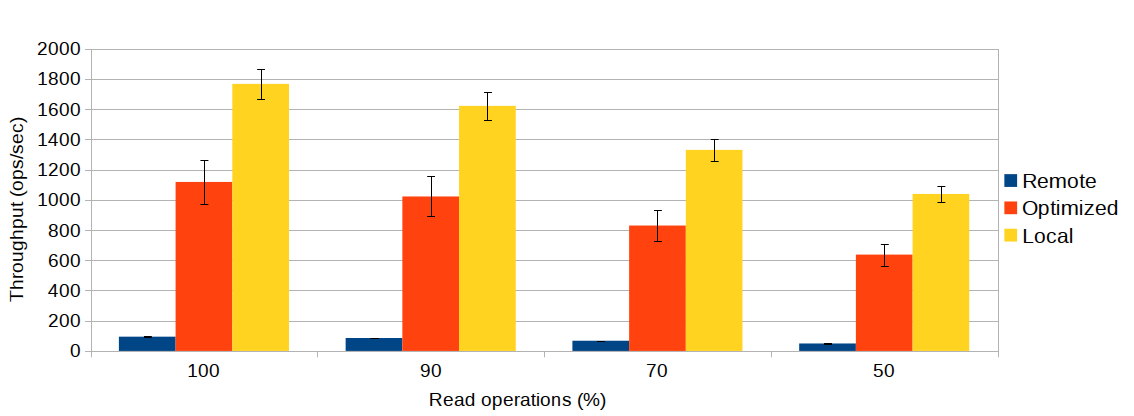
\includegraphics[width=\textwidth]{images/Uniform-dist-throughput.png}
\centering
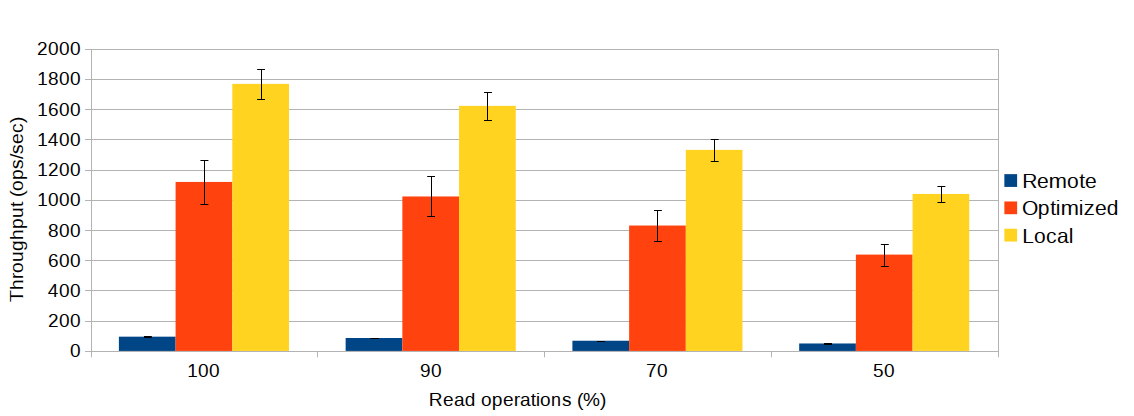
\includegraphics[scale=0.60]{images/Uniform-dist-throughput.png}
\caption{Uniform Object Access Distribution}
\label{fig:res-unif}
\end{figure*}

\begin{figure*}[ht]
% 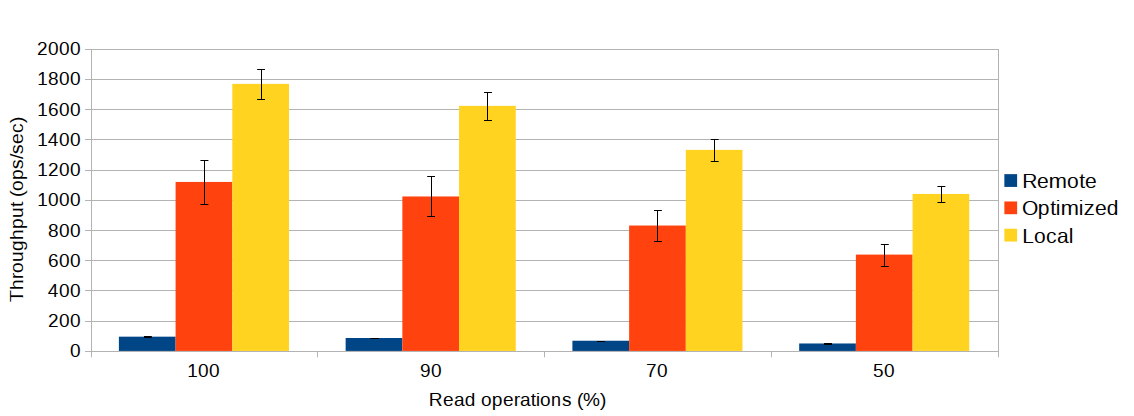
\includegraphics[width=\textwidth]{images/Uniform-dist-throughput.png}
\centering
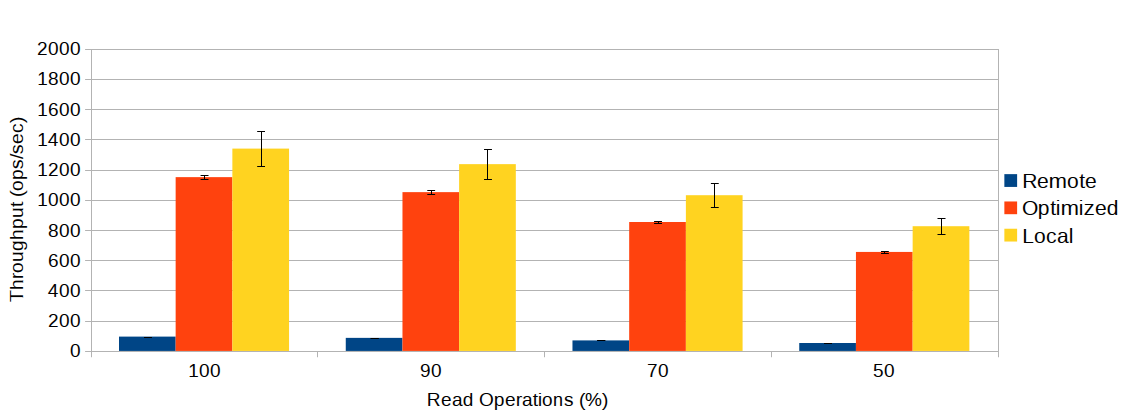
\includegraphics[scale=0.60]{images/Skewed-dist-throughput.png}
\caption{Skewed Object Access Distribution}
\label{fig:res-skew}
\end{figure*}

\subsection{Testbed}

\subsubsection{Service Infrastructure} \label{Service-Infrastructure}
The testing for this experiment was done on a cluster of 3 nodes, with 12 CPU cores and 16 GB of main memory.
Each of these nodes contains a deployment setup as follows:
\begin{itemize}
	\item RedynisService \cite{redynis-svc}
	\item Redis instance (as the actual key-value store)
	\item Redis instance (as the metadata store)
\end{itemize}

Of these, one of these nodes are randomly configured to be the master propagator, in order to serialize write transactions and ensure correctness of value data across the Redis instances.

\subsubsection{Placement Infrastructure}
A single node will be running a continuous execution for RedynisDaemon \cite{redynis-daemon}
The node's hardware specifications the same as the nodes running the service infrastucture (\ref{Service-Infrastructure}).

\subsection{Workloads}
The YCSB workloads for RESTful web-services is being used to benchmark this experimental setup.\\

The tests run were permutations of the below configurations:

\begin{itemize}
	\item  Workload Read requests (\%) ranging from 100 (all reads) to 50 (write-heavy)
	\item  Uniform key-value access distribution vs Skewed (zipfian) key-value access distribution
\end{itemize}

All of the workloads have been run on a uniform set of 1,000,000 total requests. To simulate a widely geo-distributed network of nodes, the incurred latency for making a request to a remote node is set at 100ms\cite{latency-stats}, whereas there is no incurred penalty for making a local request.

\section{Experimental Results}

The experimental results for uniform distribution of object access and skewed distribution are indicated in Figure \ref{fig:res-unif} and Figure \ref{fig:res-skew} respectively.\\

Each of the bars plotted have additional error bars to indicate the 99\% confidence interval for the distribution across the 3 iterations of the experiment performed. \\

The different scenarios enumerated in the graphs are described below:
\begin{itemize}
	\item \textbf{Local:} All requests for keys made are served by the key-value store on the local node
	\item \textbf{Remote:} All requests for keys made are served not available on the local key-value store, and for each request, the penalty of having to retrieve the key's value from a remote node, is incurred.
	\item \textbf{Optimized:} All requests for keys made are served not available on the local key-value store. However, as the requests keep coming, the usage statistics are logged, and the RedynisDaemon, following the Ownership coefficient policy detailed earlier, replicates the keys to the local key-value store on the fly, to mitigate the penalty incurred by having to make remote requests for a frequently accessed key.
\end{itemize}

The ideal outcome of the experiment was to prove that the optimized option is a good-enough alternative to a blind global replication of all keys across all nodes in the key-value cluster, and the experimental results corroborate this hypothesis.


\section{Conclusions}


\section{Acknowledgments}


\bibliographystyle{abbrv}
\bibliography{cs848-course-project_vineet.bib}


\end{document}
